\chapter{Resultados}
\label{cap:resultados}

\section{Resultados Esperados}
\label{sec:protocolo_resultados}

Para obtenção dos resultados é estabelecido um protocolo de uso dos modelos discutidos no capítulo de Materiáis e métodos \ref{cap:materiais_e_metodos}, sumarizados a seguir:

\begin{outline}[enumerate]
    \1 É executado o algoritmo \textbf{auto ARIMA} para obtenção do modelo SARIMAX, com frequência sazonal 24 e todas as variáveis exógenas destacadas na seção \ref{subsec:orig_data} fazendo parte da regressão.
    \1 É executado o algoritmo PSO-ACO SARIMAX.
        \2 Tendo como limite máximo de dimensionalidade para os parâmetros (p,d,q) e (P, D, Q) uma unidade acima do encontrado pelo modelo resultante do \textbf{auto ARIMA}.
        \2 A Sazonalidade é com frequência entre 24 e 48.
        \2 As variáveis exógenas são testadas para saber quais destas de fato ajudam o modelo.
            \3 Precipitação Total (mm)
            \3 Temperatura do Ar (\textdegree{}C)
            \3 Umidade Relativa (\%)
            \3 Velocidade do Vento (m/s)
            \3 Velocidade do Vento em rajada (m/s)
        \2 Se o resultado for pior que o obtido pelo \textbf{auto ARIMA}, este último é mantido. A comparação é feita a partir da métrica AICc.
    \1 O modelo SARIMAX selecionado segue para uso nos modelos híbridos descritos nas subseções \ref{subsec:ag-mlp} e \ref{subsec:ag-mlp-vr}.
        \2 Para todas as séries foi estipulado 80\% de dados para treino, que são utilizados para realizar o treinamento do algoritmo de otimização e hibridização, bem como todas as MLPs e 20\% para teste, que utilizado para avaliação do modelo híbrido final.
\end{outline}

Com base neste protocolo de uso do algoritmos propostos, nas próximas seções são apresentados resultados parciais para algumas cidades brasileiras escolhidas. Espera-se que os resultados finais sigam o mesmo padrão observado nos parciais, porém para mais localidades.

\section{Resultados Parciais}

\subsection{Maceió}

Maceió - AL é a cidade escolhida para primeiro resultado preliminar do protocolo definido. O conjunto de dados para esta cidade, se trata de 30 dias, entre 12/03/2020 às 21 horas e 11/04/2020 às 20 horas da base para a cidade de Maceió-AL. Esta localidade foi escolhida por conta da proposta do projeto de pesquisa e desenvolvimento realizado para a CHESF, também sendo importante destino turístico regional, destacando-se o "turismo de sol e mar" \cite{vasconcelos2019turismo}. A Tabela \ref{tab:cap4_comp_maceio_autoarima_psoaco} mostra o resultado da comparação entre os algoritmos descritos na seção \ref{subsec:autoarima_psoaco}. 

\begin{table}[htbp]
\caption{Comparação resultados entre \textbf{auto ARIMA} e PSO-ACO.}
\begin{center}
\begin{tabular}{ccccc}
                    & \Longstack{SARIMAX \\ (p,d,q)(P,D,Q,S)} & Variáveis Exógenas & AICc & MAPE  \\\hline
auto ARIMA & (1,0,2)(1,0,2,24) & Todas & -1488.858 & \textbf{5.3497} \\\hline
PSO-ACO             & (2,0,0)(1,0,1,24) & Temperatura do Ar & \textbf{-1516.263} & 6.7475 \\\hline
\label{tab:cap4_comp_maceio_autoarima_psoaco}
\end{tabular}
\end{center}
\end{table}

Como descrito no início do capítulo, e pelo que foi obtido, optou-se por utilizar a modelagem SARIMAX obtida descrita na segunda linha da Tabela \ref{tab:cap4_comp_maceio_autoarima_psoaco}, como entrada para os algoritmos híbridos descritos pela seções \ref{subsec:ag-mlp} e \ref{subsec:ag-mlp-vr}, resultando finalmente nos resultados descritos pela Tabela \ref{tab:cap4_comp_maceio_agmlp_agmlpvr}.Para ambos os algoritmos foram utilizadas 3 gerações e 12 indivíduos.

\begin{table}[htbp]
\caption{Comparação entre modelos para aos dados da cidade de Maceió-AL}
\begin{center}
\begin{tabular}{ccccc}
                & MAE & MSE & MAPE \\\hline
SARIMAX         & 0.035221 & 0.002941 & 2.91303 \\\hline
Híbrido AG-MLP  & \textbf{0.024321} & \textbf{0.001857} & 0.90901 \\\hline
Híbrido AG-MLP-VR & 0.02684 & 0.002439 & \textbf{0.530453} \\\hline
\label{tab:cap4_comp_maceio_agmlp_agmlpvr}
\end{tabular}
\end{center}
\end{table}

Um resultado gráfico para a localidade definida pode ser observado na Figura \ref{fig:cap4_maceio_3_days_hibrids} em que se mostra as 3 formas de modelagem e o seu resultado sobre as últimas 72 horas de dados.

\begin{figure}[!htbp]
    \centering
    \caption{Últimas 72 horas do resultado utilizando algoritmos AG-MLP e AG-MLP-VR, SARIMAX e série real. Para a cidade de Maceió-AL}
    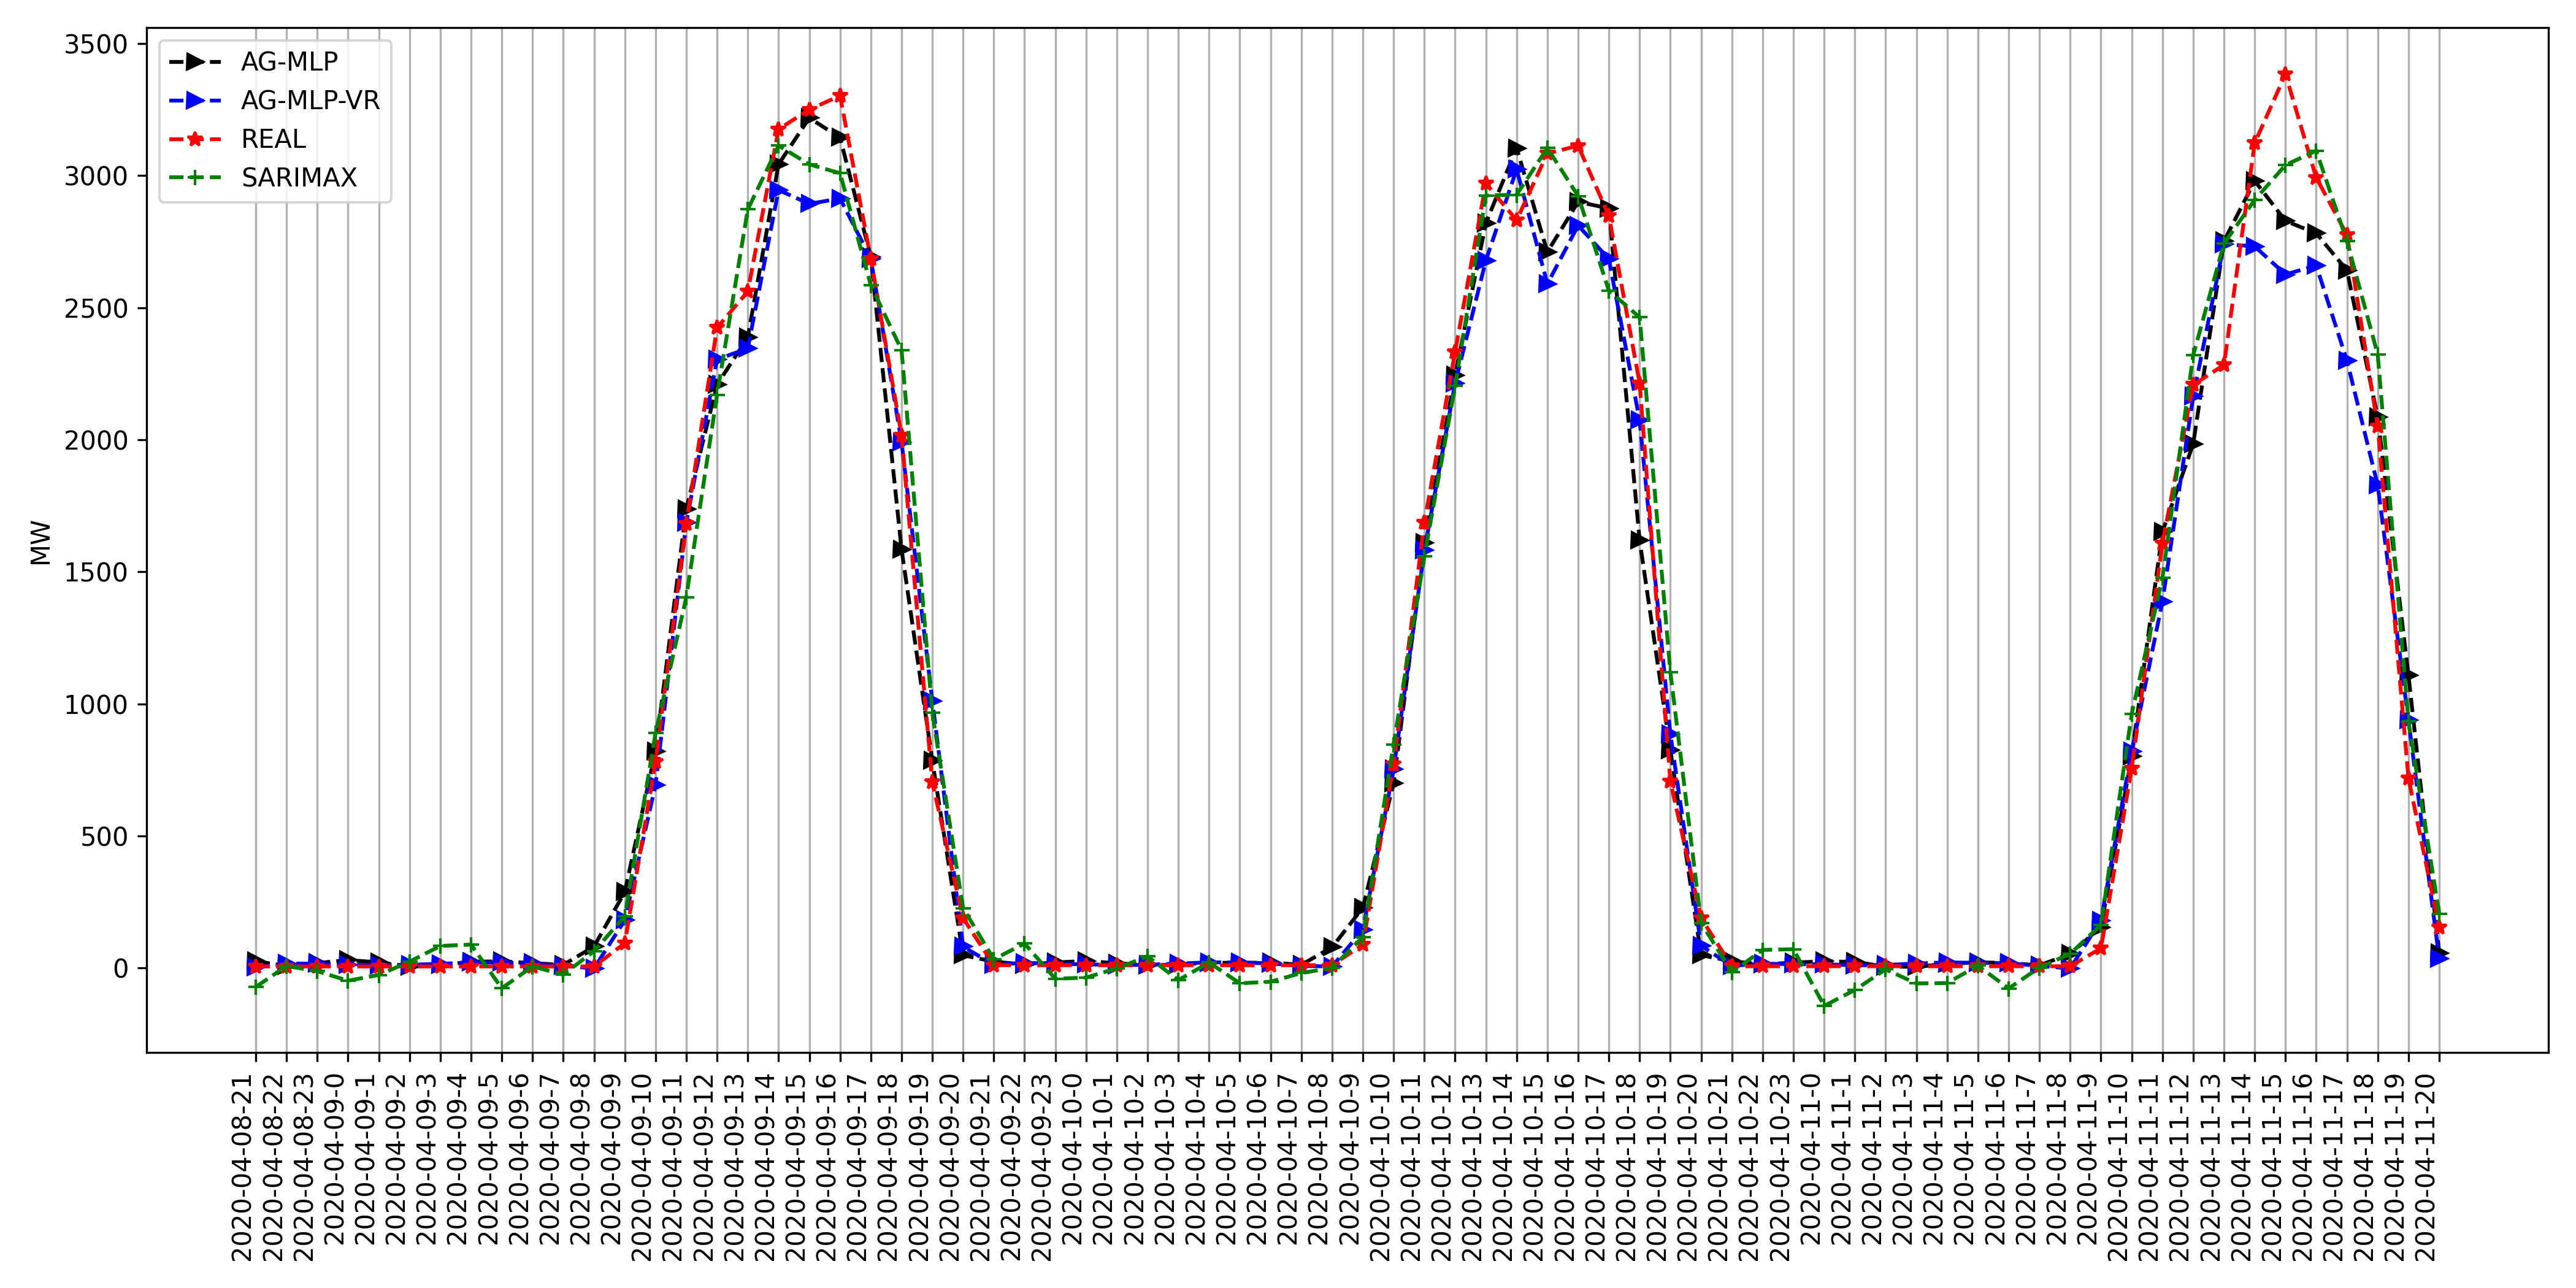
\includegraphics[width=\textwidth]{Figuras/results/comparison_hibrids_mc.png}
    \source{Autor.}
    \label{fig:cap4_maceio_3_days_hibrids}
\end{figure}

\subsection{Florianópolis}

Tendo uma região metropolitana importante economicamente, com atrativos ecoturísticos, Florianópolis-SC, foi escolhida para integrar os resultados \cite{bittencourt2015ecoturismo, cavanus2021sapiens}. Se tratando da segunda série temporal que será apresentada nos resultados deste trabalho.

São utilizados os últimos 15 dias da base obtida, entre 17/12/2019 às 0 horas e 31/12/2019 às 23 horas. A Tabela \ref{tab:cap4_comp_flor_autoarima_psoaco} mostra o resultado da comparação entre os algoritmos descritos na seção \ref{subsec:autoarima_psoaco}.

\begin{table}[htbp]
\caption{Comparação resultados entre \textbf{auto ARIMA} e PSO-ACO.}
\begin{center}
\begin{tabular}{ccccc}
                    & \Longstack{SARIMAX \\ (p,d,q)(P,D,Q,S)} & Variáveis Exógenas & AICc & MAPE  \\\hline
auto ARIMA & (0,1,1)(2,0,2,24) & Todas & -695.210 & \textbf{57.106} \\\hline
PSO-ACO             & (2,0,2)(1,0,1,24) & \Longstack{Temperatura do Ar \\ Precipitação} & \textbf{-754.4754} & 52.316 \\\hline
\label{tab:cap4_comp_flor_autoarima_psoaco}
\end{tabular}
\end{center}
\end{table}

Como descrito no início do capítulo, e pelo que foi obtido, optou-se por utilizar a modelagem SARIMAX obtida descrita na segunda linha da Tabela \ref{tab:cap4_comp_flor_autoarima_psoaco}, como entrada para os algoritmos híbridos descritos pela seções \ref{subsec:ag-mlp} e \ref{subsec:ag-mlp-vr}, resultando finalmente nos resultados descritos pela Tabela \ref{tab:cap4_comp_flor_agmlp_agmlpvr}.Para ambos os algoritmos foram utilizadas 3 gerações e 12 indivíduos.

\begin{table}[htbp]
\caption{Comparação entre modelos para aos dados da cidade de Florianópolis-SC}
\begin{center}
\begin{tabular}{ccccc}
                & MAE & MSE & MAPE \\\hline
SARIMAX         & 0.03370 & 0.00278 & 7.6349 \\\hline
Híbrido AG-MLP  & \textbf{0.01665} & \textbf{0.000818} & 1.90307 \\\hline
Híbrido AG-MLP-VR & 0.023722 & 0.00240 & \textbf{0.93862} \\\hline
\label{tab:cap4_comp_flor_agmlp_agmlpvr}
\end{tabular}
\end{center}
\end{table}

Novamente, é apresentado um resultado gráfico na Figura \ref{fig:cap4_flor_3_days_hibrids} em que se mostra as 3 formas de modelagem e o seu resultado sobre as últimas 72 horas de dados.

\begin{figure}[!htbp]
    \centering
    \caption{Últimas 72 horas do resultado utilizando algoritmos AG-MLP e AG-MLP-VR, SARIMAX e série real. Para a cidade de Florianópolis-SC}
    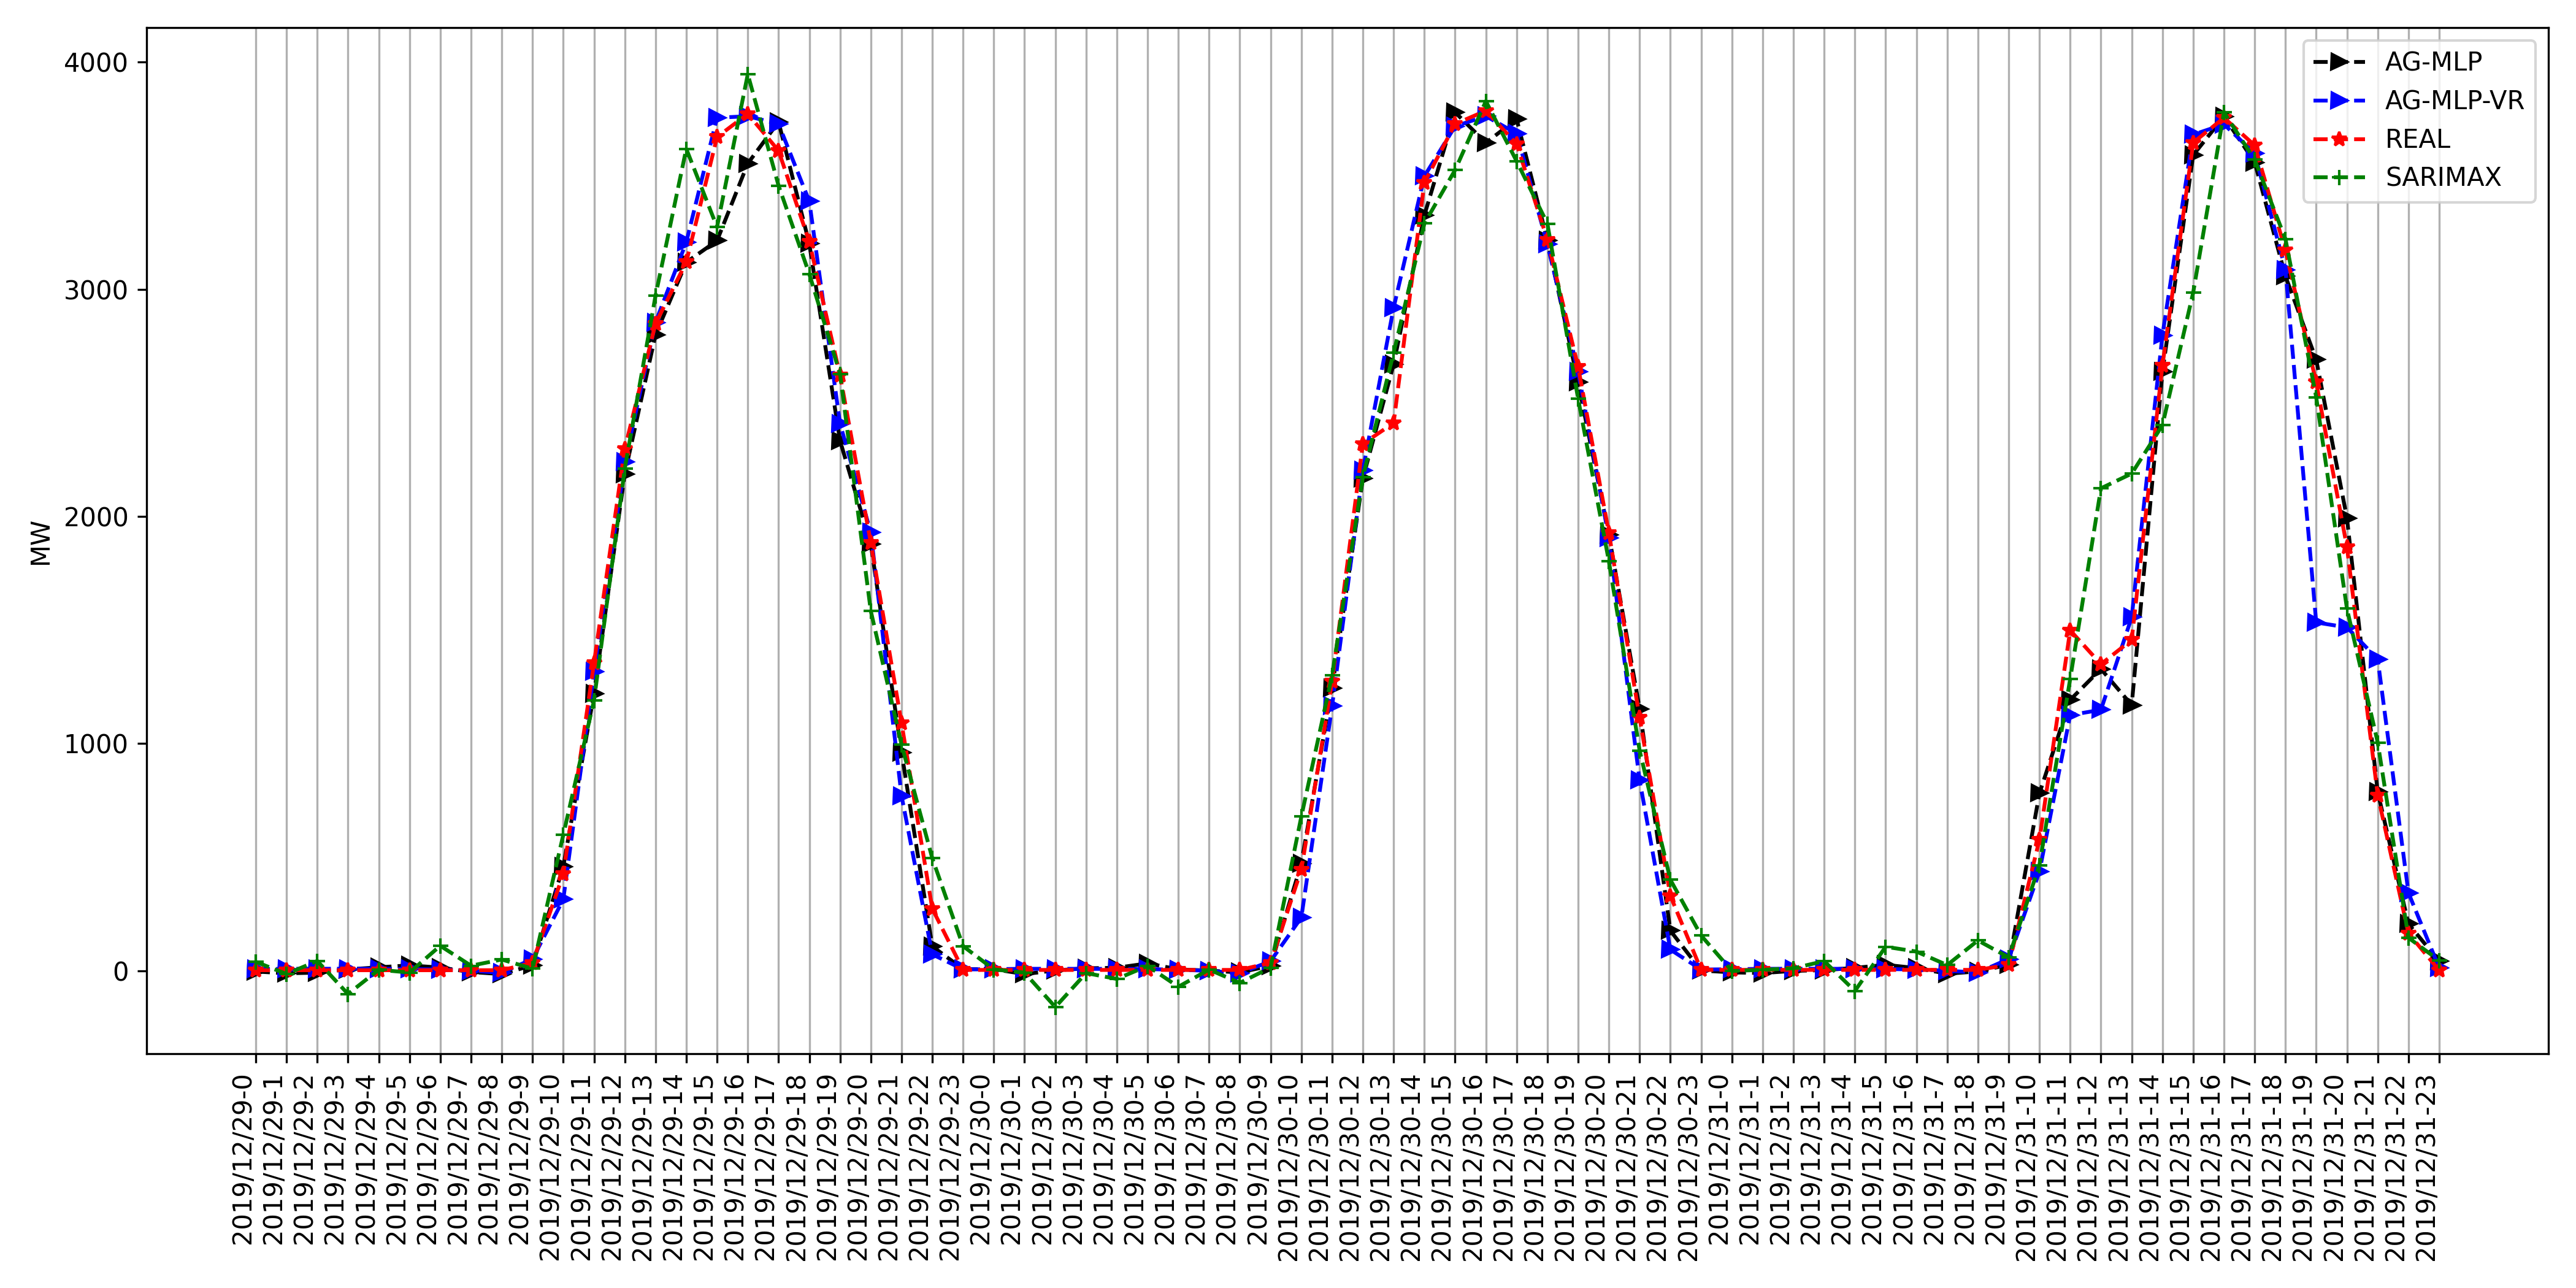
\includegraphics[width=\textwidth]{Figuras/results/comparison_hibrids_fl.png}
    \source{Autor.}
    \label{fig:cap4_flor_3_days_hibrids}
\end{figure}

\subsection{Bom Jesus da Lapa}

A terceira série temporal escolhida se trata de 15 dias, entre 17/07/2020 às 0 horas e 31/07/2020 às 23 horas da base para a cidade de Bom Jesus da Lapa - BA. Esta localidade foi escolhida por conter plantas fotovoltaicas próximas e ser um dos pontos de maior incidência de radiação fotovoltaica de acordo com o Atlas solarimétrico brasileiro \cite{pereira2017atlas}. A Tabela \ref{tab:cap4_comp_bjl_autoarima_psoaco} mostra o resultado da comparação entre os algoritmos descritos na seção \ref{subsec:autoarima_psoaco}.

\begin{table}[htbp]
\caption{Comparação resultados entre \textbf{auto ARIMA} e PSO-ACO.}
\begin{center}
\begin{tabular}{ccccc}
                    & \Longstack{SARIMAX \\ (p,d,q)(P,D,Q,S)} & Variáveis Exógenas & AICc & MAPE  \\\hline
auto ARIMA & (3,0,2)(2,0,2,24) & Todas & -825.1507 & 0.9518 \\\hline
PSO-ACO             & (1,0,0)(2,0,2,24) & \Longstack{Temperatura do Ar \\ Umidade Relativa \\ Velocidade do Vento} & \textbf{-831.802} & \textbf{0.9233} \\\hline
\label{tab:cap4_comp_bjl_autoarima_psoaco}
\end{tabular}
\end{center}
\end{table}

Como descrito no início do capítulo, e pelo que foi obtido, optou-se por utilizar a modelagem SARIMAX obtida descrita na segunda linha da Tabela \ref{tab:cap4_comp_bjl_autoarima_psoaco}, como entrada para os algoritmos híbridos descritos pela seções \ref{subsec:ag-mlp} e \ref{subsec:ag-mlp-vr}, resultando finalmente nos resultados descritos pela Tabela \ref{tab:cap4_comp_bjl_agmlp_agmlpvr}. Para ambos os algoritmos foram utilizadas 4 gerações e 15 indivíduos.

\begin{table}[htbp]
\caption{Comparação entre modelos para aos dados da cidade de Florianópolis-SC}
\begin{center}
\begin{tabular}{ccccc}
                & MAE & MSE & MAPE \\\hline
SARIMAX         & 0.03115 & \textbf{0.00252} & 0.3486 \\\hline
Híbrido AG-MLP  & \textbf{0.03105} & 0.00304 & \textbf{0.19175} \\\hline
Híbrido AG-MLP-VR & 0.03224 & 0.002783 & 0.25194 \\\hline
\label{tab:cap4_comp_bjl_agmlp_agmlpvr}
\end{tabular}
\end{center}
\end{table}

Por fim, pode ser visto na Figura \ref{fig:cap4_bjl_3_days_hibrids} um exemplo da diferença entre as séries, em que se mostra as 3 formas de modelagem e o seu resultado sobre as últimas 72 horas de dados.

\begin{figure}[!htbp]
    \centering
    \caption{Últimas 72 horas do resultado utilizando algoritmos AG-MLP e AG-MLP-VR, SARIMAX e série real. Para a cidade de Bom Jesus da Lapa - BA}
    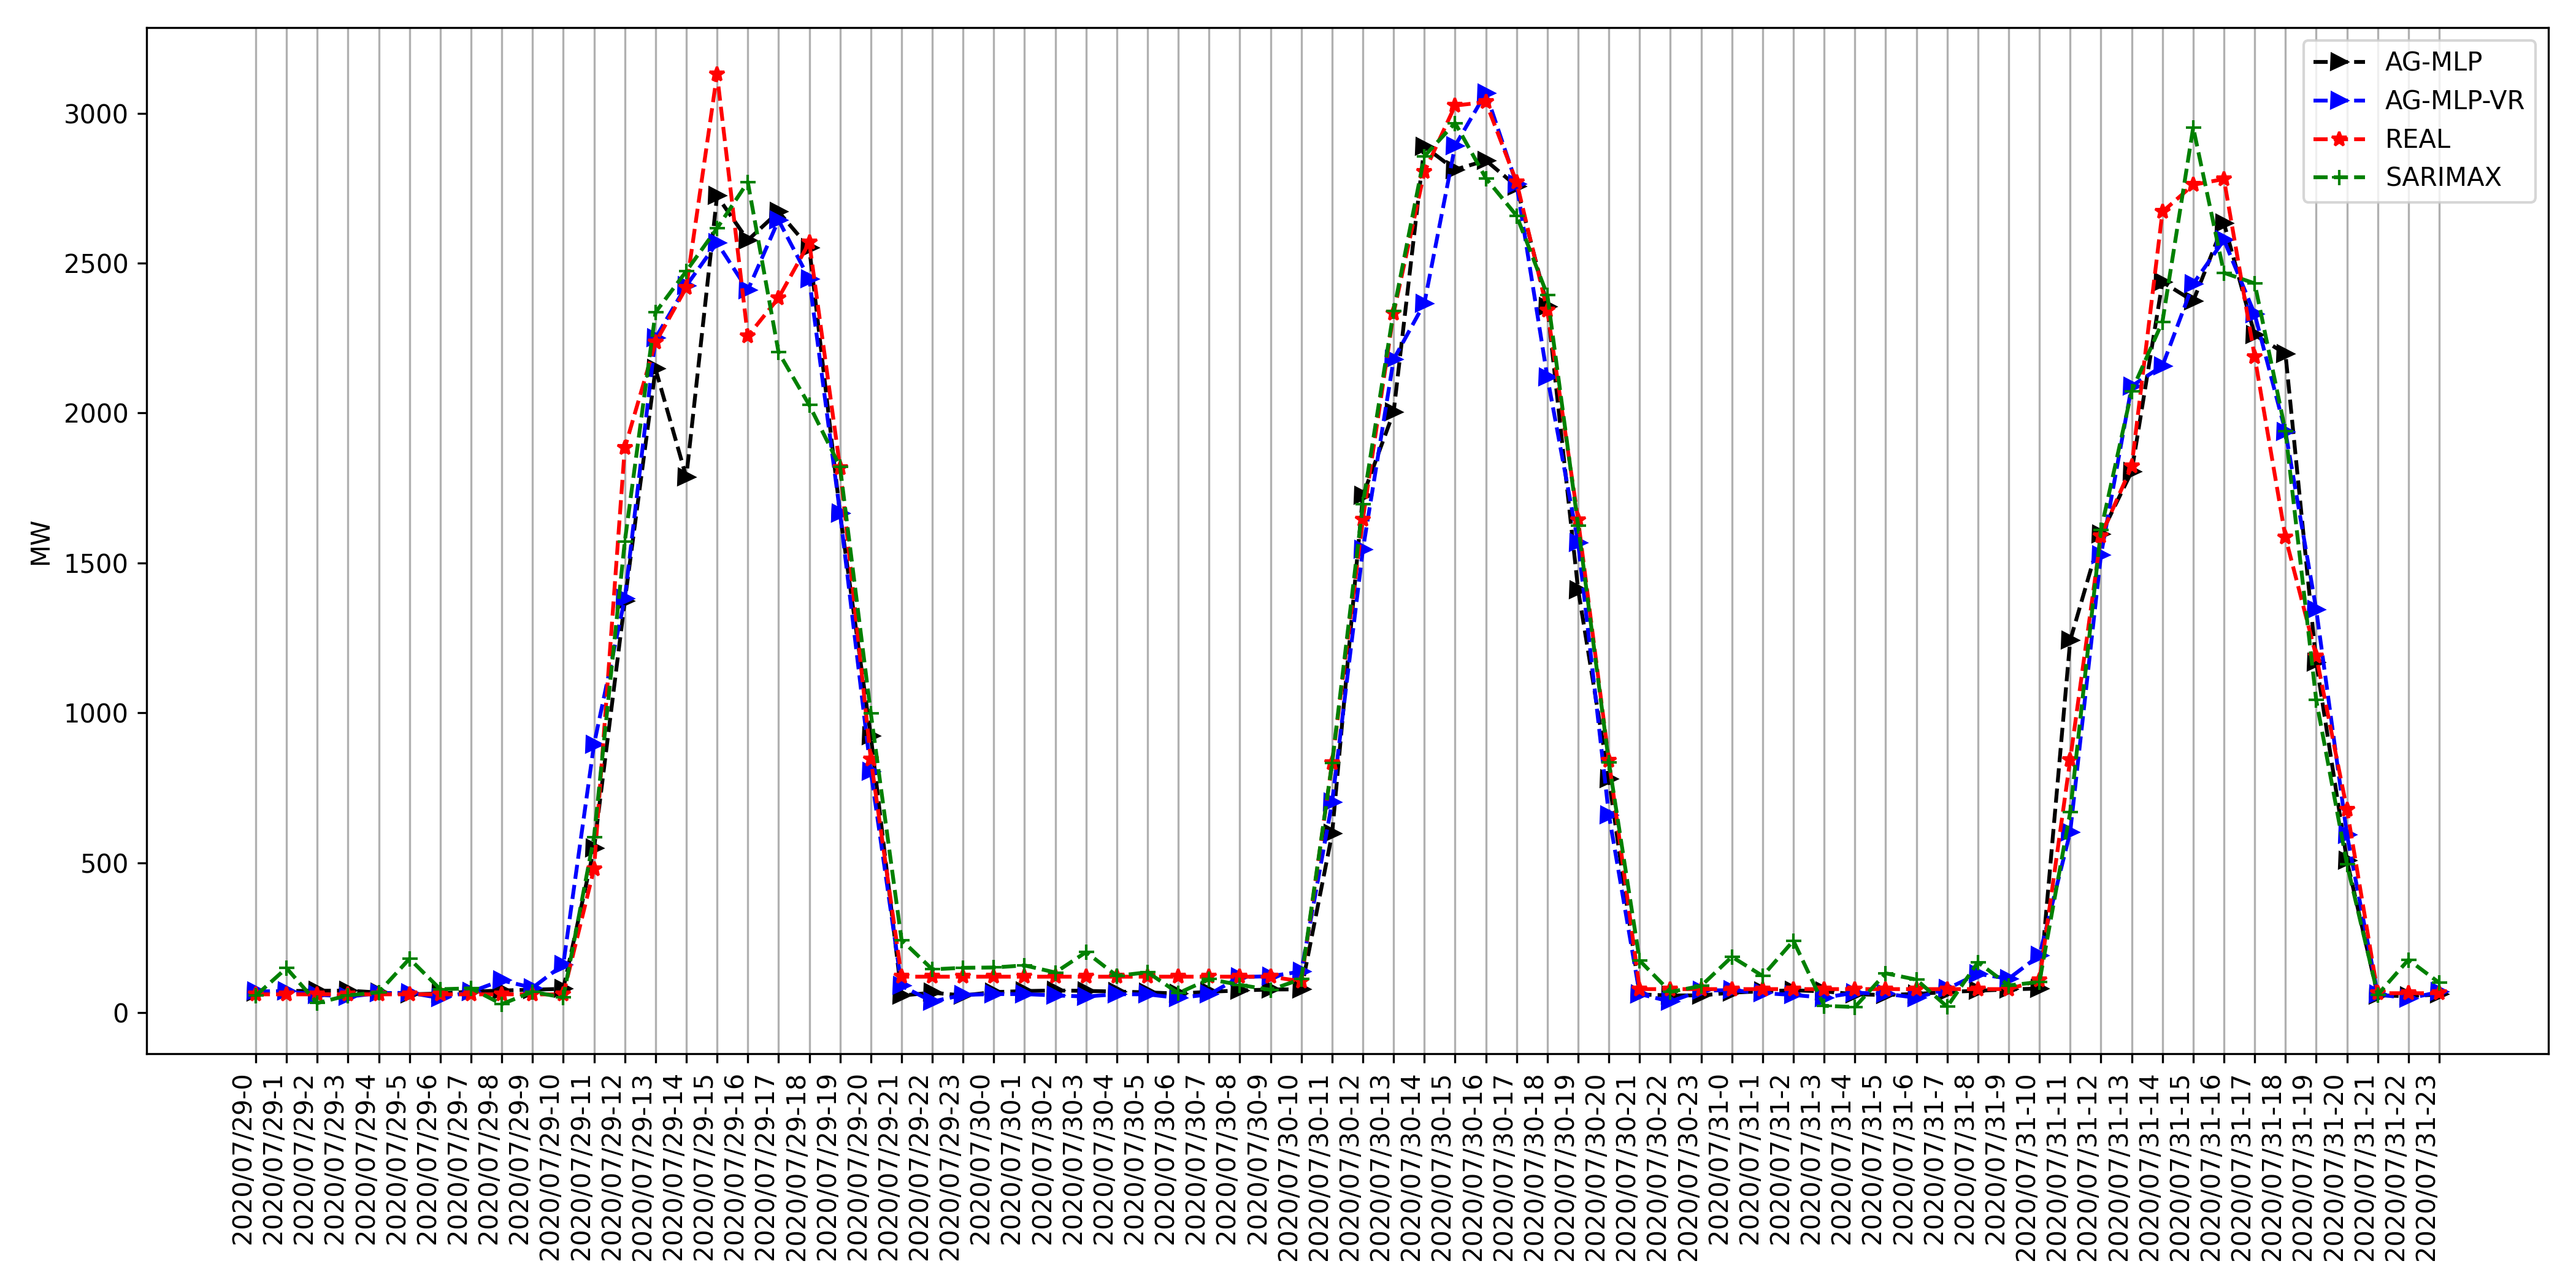
\includegraphics[width=\textwidth]{Figuras/results/comparison_hibrids_bjl.png}
    \source{Autor.}
    \label{fig:cap4_bjl_3_days_hibrids}
\end{figure}

